\chapter{Opis projektnog zadatka}
		
		Cilj ovog projekta je razviti programsku podršku za stvaranje web aplikacije "\textit{StreetPatrol}". Ideja aplikacije je ponuditi običnim građanima jednostavan i efikasan način prijave oštećenja javnih površina i cesta u gradu te dobivanje povratnih informacija o konkretnom oštećenju i njihovoj prijavi. 
		
		Građani će svojim djelovanjem putem aplikacije unaprjeđivati kvalitetu života u svojoj zajednici. Svojim prijavama, koje će biti javno dostupne, građani će poticati gradske urede da saniraju prijavljena oštećenja. Aplikacija će također pomoći gradskim uredima u obavljanju svojih zadaća. Naime, preko aplikacije uredi će imati puno bolji uvid u probleme koji postoje u zajednici. Zahvaljujući aplikaciji uredi će moći brže i kvalitetnije reagirati na probleme u zajednici.
		
		\underbar{Građani} aplikaciju mogu koristiti kao registrirani i kao neregistrirani korisnici. Građani imaju mogućnost podnošenja nove prijave, pregleda postojećih prijava i pregled statistike prijava. Registrirani građani također imaju opciju pregleda svojeg profila dok neregistrirani građani imaju mogućnost registracije, tj. izrade profila odnosno prijave, ako već imaju izrađeni profil.
		
		Neregistrirani korisnik se može registrirati te prilikom registracije mora navesti sljedeće informacije:
		\begin{packed_item} 
			\item ime
			\item prezime
			\item email adresa
			\item lozinka
		\end{packed_item}  
		Prijavljeni korisnici prilikom pregleda svojeg profila mogu vidjeti prije navedene podatke o sebi koje mogu i izmijeniti. Također imaju pregled nad svim prijavama koje su podnesli kroz aplikaciju. Prikazana im je i kratka statistika prijava (broj prijava, broj riješenih prijava, broj prijava na čekanju i u procesu rješavanja). 
		
		Građanima se prilikom podnošenja nove prijave otvara obrazac koji je potrebno ispuniti. Prijava sadrži naslov, kratak opis, lokaciju i kategoriju oštećenja. Opcionalno se u prijavi može priložiti fotografija oštećenja. Lokacija oštećenja se prilaže odabirom položaja na karti ili upisivanjem adrese na kojoj se nalazi oštećenje. Ako korisnik priloži fotografiju, aplikacija će pokušati iz nje izvući podatke o lokaciji te ih ponuditi korisniku kao lokaciju oštećenja. Odabirom kategorije oštećenja korisnik indirektno odabire gradski ured nadležan za konkretan problem. Prilikom opisivanja oštećenja aplikacija će pokušati sama zaključiti kojoj kategoriji oštećenje pripada te će istu predložiti korisniku. Također, ako u sustavu već postoji slična nedavna prijava na istoj lokaciji aplikacija će predložiti korisniku postojeću prijavu i ponuditi mu da svoju prijavu nadoveže na postojeću. Nakon podnošenja prijave aplikacija korisniku daje jedinstveni kod podnesene prijave koja služi za praćenje te prijave preko same aplikacije. Prijavljeni korisnici će također primati obavijesti o svojoj prijavi preko emaila.
		
		Za pregled postojećih prijava korisnik koristi interaktivnu kartu s označenim prijavama na njoj. Prijave se mogu dodatno filtrirati po vremenu podnošenja prijave, statusu, kategoriji oštećenja i nadležnom gradskom uredu. Korisnik također može pretraživati prijave po jedinstvenom kodu prijave. Na taj način svaki korisnik može pregledavati svoje prijave na aplikaciji. Odabirom neke prijave prikazuju se podaci iz podnesenog obrasca o odabranoj prijavi. Također se prikazuje status prijave (\textit{na čekanju}, \textit{u procesu rješavanja}, \textit{riješena}), broj prijava koje su vezane za ovu prijavu, odnosno prijava za koju je vezana ova prijava. Prijavljeni korisnici također vide svoje prijave na pregledu svojeg profila. Prijave koje su riješene mogu se pregledati jedino preko njihovog koda ili preko pregleda korisničkog profila kod registriranih korisnika. U drugim slučajevima takve prijave nisu više dostupne za pregled.
		
		Prikaz statistike prijava nudi filtriranje podataka po vremenu podnošenja prijave, kategoriji oštećenja i nadležnom gradskom uredu. Za odabrane parametre aplikacija prikazuje:
		\begin{packed_item} 
			\item ukupan broj podnesenih prijava
			\item broj prijava sa statusom \textit{na čekanju} i njihov udio
			\item broj prijava sa statusom \textit{u procesu rješavanja} i njihov udio
			\item broj prijava sa statusom \textit{riješena} i njihov udio
			\item prosječan broj podnesenih prijava u danu
			\item prosječan broj dana koji prijava provede na čekanju
			\item prosječan broj dana za vrijeme kojih je prijava u procesu rješavanja
		\end{packed_item}
		
		\underbar{Djelatnici gradskog ureda} se obavezno u sustav prijavljuju preko profila gradskog ureda. Djelatnici pregledavaju prijave kroz 3 liste, jedna za svaku vrstu statusa: novopristigle, one u procesu rješavanja i riješene prijave. Djelatnici ureda imaju isključivo pristup prijavama za oštećenja za koja je nadležan njihov ured. Ostale prijave djelatnicima nisu vidljive.
		
		Sustav nudi mogućnost registracije novih gradskih ureda. U tom slučaju kod stranice za registraciju potrebno je odabrati opciju registracije gradskog ureda. Aplikacija tada prikazuje obrazac za koji je potrebno navesti:
		\begin{packed_item} 
			\item ime gradskog ureda
			\item email adresa gradskog ureda
			\item lozinka za račun gradskog ureda
			\item jedna ili više kategorija koje će novi gradski ured pokrivati
		\end{packed_item}
		
		Djelatnici pregledavaju pristigle prijave i stavljaju ih u proces rješavanja. Time prijave prelaze u listu prijava u procesu rješavanja i mijenjaju svoj status. Aplikacija u tom slučaju automatski šalje obavijest prijavitelju ako se radi o registriranom korisniku.
		
		Kada neka prijava bude riješena, djelatnik prijavi mijenja status u \textit{riješena}. Prijava prelazi u za to predviđenu listu te aplikacija šalje obavijest prijavitelju ako se radi o registriranom korisniku.
		
		Prethodne dvije radnje bi trebale sadržavati komunikaciju s nadležnim gradskim službama. Dakle, po primitku prijave djelatnik promjenom statusa prijave delegira prijavu nadležnoj gradskoj službi. Kada nadležna služba riješi problem šalje informaciju uredu koji onda može prijavu označiti kao riješenu. Ova funkcionalnost nije implementirana jer zahtjeva komunikaciju s vanjskim sustavima što nije u opsegu ovog projekta.
		
		Djelatnik ima mogućnost objedinjavanja prijava. Naime, ako se pristigla prijava referira na problem za koji već postoji prijava, djelatnik može grupirati te prijave. Aplikacija u tom slučaju šalje prikladnu obavijest registriranim korisnicima čije su prijave zahvaćene ovom radnjom.
		
		Ako procijeni da je pristigla prijava poslana na krivi ured, djelatnik ima mogućnost proslijediti prijavu uredu koji je zapravo nadležan za pristiglu prijavu. Korisniku koji je podnio prijavu se u tom slučaju šalje prikladna obavijest putem maila ako je taj korisnik registriran.
		
		Slično, ako procijeni da pristigla prijava uopće nije valjana, djelatnik ima mogućnost odbaciti prijavu. U tom slučaju se prijava arhivira u bazi podataka ali se više ne koristi. Korisnik koji je podnio prijavu dobiva prikladnu obavijest putem maila ako je registriran.
		
		Djelatnici gradskih ureda mogu pregledavati statistiku prijava kao i obični korisnici, uz restrikciju na prijave vezane na njihov ured, kao što je prije navedeno.
		
		Aplikacija je napravljena tako da podržava višejezičnost. Aplikacija podržava hrvatski i engleski jezik.
		
		Aplikacija je napravljena na primjeru Grada Zagreba. Karte u aplikaciji će prikazivati područje Grada Zagreba i prijave će se moći podnositi samo za oštećenja u tom području. Aplikacija nema fiksirani broj gradskih ureda, već je omogućeno dodavanje novih ureda, Kao što je već i navedeno. Time je aplikaciju lakše prilagoditi promjenama u organizaciji gradskih ureda. Također, na ovaj način je lakše konfigurirati aplikaciju za implementaciju u nekom drugom području osim Grada Zagreba.
		\eject
		
		\section{Postojeća rješenja za slični problem}
		
			Slične aplikacije već postoje u Hrvatskoj. Tako primjerice Grad Rijeka na svojim stranicama nudi mogućnost prijave raznih prekršaja i oštećenja (\url{https://gov.rijeka.hr/zahtjevi-i-obrasci/komunalna-djelatnost-i-prijava-komunalnog-nereda/prijave-ostecenja-nereda-ili-nepropisnog-parkiranja/383}). Njihova stranica nudi mogućnost prijave u 4 kategorije. Neke prijave se podnose putem obrazaca, neke samo telefonskim putem, a za neke su ponuđene i specijalne stranice. Tako primjerice za prijavu većine problema, ali i za podnošenje pohvala, Grad Rijeka nudi web aplikaciju \textit{Gradsko oko} (\url{http://rijeka.oko.hr/}) dostupnu i u mobilnoj verziji. Aplikacija nudi mogućnost podnošenja i pregleda prijava putem interaktivne karte. Prijave su kategorizirane po grupama i klasifikacijama. Prilikom pregleda se mogu filtrirati po vremenu i kategorijama. Prijave i pregled prijava su dostupne samo prijavljenim korisnicima te svaka prijava mora biti odobrena od strane administratora.
		
		\begin{figure}[H]
			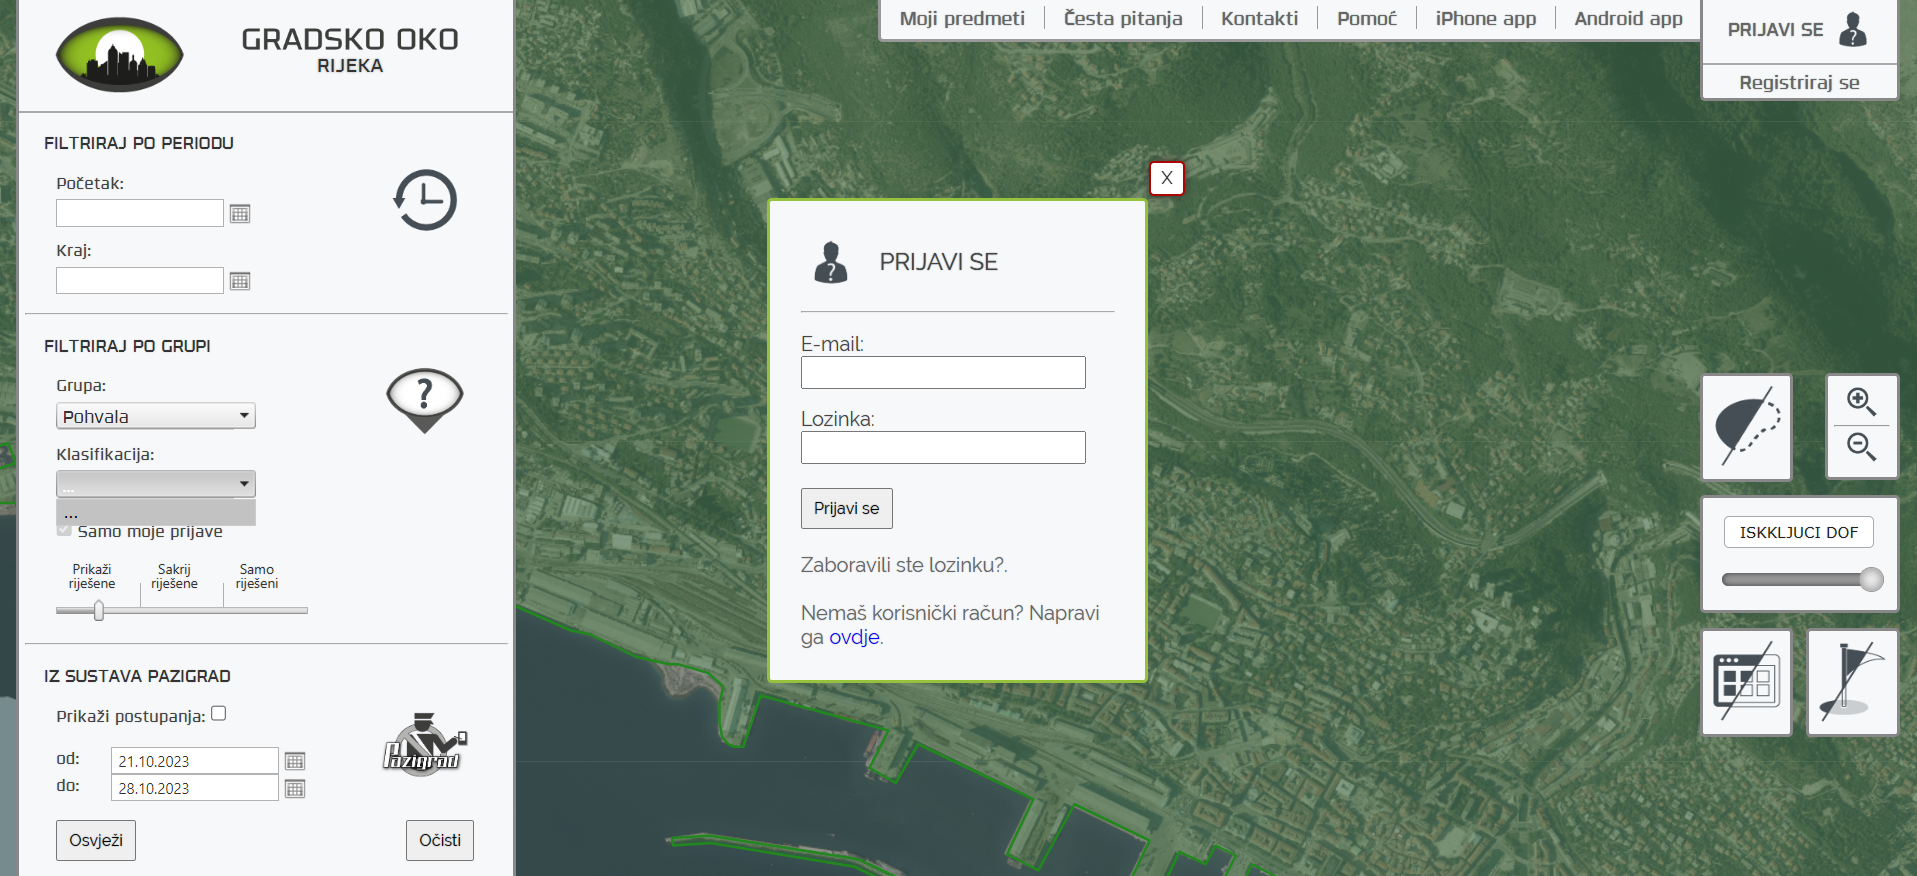
\includegraphics[width=\textwidth]{slike/GradskoOko.PNG}
			\caption{Aplikacija \textit{Gradsko oko} Grada Rijeke}
			\label{fig:gradskooko} %label mora biti drugaciji za svaku sliku
		\end{figure}
		
		\eject
		
		\section{Mogućnosti nadogradnje i skaliranja rješenja} 
		
		Uz male preinake moguće je prilagoditi aplikaciju da pruža istu potporu građanima nekog drugog grada ili općine, bilo u Hrvatskoj ili nekoj drugoj zemlji. Aplikacija bi se mogla skalirati i na veće jedinice lokalne samouprave kao što su županije, s obzirom na to da obično imaju sličan ustroj ureda i slične nadležnosti kao i gradovi. Ako se ideja skalira još više, aplikacija bi mogla pružati uslugu korisnicima cijele regije (npr. Slavonija, Dalmacija, Središnja Hrvatska) ili čak čitave države. U tom slučaju u aplikaciji bi bilo potrebno dodati mogućnost prepoznavanja nadležne jedinice lokalne samouprave prije predlaganja nadležnog ureda za konkretan problem. Takvo ponašanje bi se moglo implementirati uz malo prerađivanja i korištenje postojećih funkcionalnosti aplikacije. Generalno gledano, aplikacija bi se mogla skalirati tako da pruža uslugu korisnicima nadnacionalnoj razini, primjerice na području cijele Europske Unije. Ponašanje aplikacije bi zapravo bilo isto uz potrebe skaliranja funkcionalnosti prepoznavanja nadležnih administrativnih jedinica na nadnacionalnoj razini. U tom slučaju aplikacija svakako mora pružati mogućnost prikaza na jeziku svake države u kojoj pruža uslugu. Glavna prepreka u ovakvoj implementaciji bi bila potreba za značajnijom infrastrukturalnom podrškom, prvenstveno u obliku velikih poslužitelja koji mogu obrađivati puno zahtjeva i pohranjivati velike količine podataka. Također, aplikacija bi na toj razini zahtijevala dobru suradnju i koordinaciju velikog broja institucija u više različitih država što može biti zahtjevno.
		
		\eject
		